\chapter{Assignment solutions-Hamilltonian Equation of Motion}
\begin{abox}
Assignment solution-1
\end{abox}
\begin{enumerate}
	\item $\left. \right. $
	\begin{answer}
		\begin{align*}
		\text{(A) }T&=\frac{1}{2} m\left(\dot{r}^{2}+r^{2} \dot{\theta}^{2}+\dot{z}^{2}\right)=\frac{m}{2}\left(\dot{r}^{2}+r^{2} \dot{\theta}^{2}+a^{2} r^{2} \dot{r}^{2}\right) \quad \because z=\frac{1}{2} a r^{2} \Rightarrow \quad \dot{z}=a r \dot{r}\\
		V&=m g z=\frac{1}{2} m g a r^{2} \\
		L&=\frac{m}{2}\left[\dot{r}^{2}\left(1+a^{2} r^{2}\right)+r^{2} \dot{\theta}^{2}-a g r^{2}\right]
	\intertext{	(a) $\theta$ is cyclic coordinate}
	\because \frac{\partial L}{\partial \theta}&=0, \Rightarrow \dot{p}_{\theta}=0 \Rightarrow P_{\theta}=\text{ constant}
	\intertext{(b) Hamiltonian}
	H&=\frac{p_{r}^{2}}{2 m\left(1+a^{2} r^{2}\right)}+\frac{p_{\theta}^{2}}{2 m r^{2}}+\frac{1}{2} m a g r^{2} \quad \\&\because \frac{\partial L}{\partial \dot{r}}=p_{r}=m\left(1+a^{2} r^{2}\right) \dot{r}\text{ and }\frac{\partial L}{\partial \dot{\theta}}=p_{\theta}=m r^{2} \dot{\theta}
		\end{align*}
	\end{answer}
	\item $\left. \right. $
	\begin{figure}[H]
		\centering
		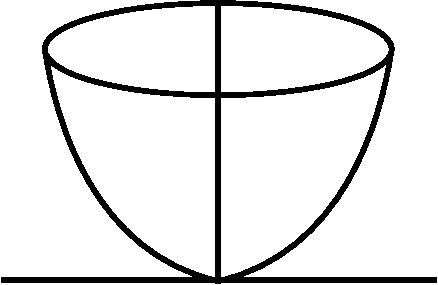
\includegraphics[height=2cm,width=3.5cm]{diagram-20220314-9-crop}
	\end{figure}
    \begin{answer}
    	\begin{align*}
    	\because z&=a\left(x^{2}+y^{2}\right)
    	\intertext{Using equation of constrain, we must solve the given system in cylindrical co-ordinate.}
    	z&=a r^{2}, \dot{z}=2 a r \dot{r}\\
    	L&=\frac{1}{2} m\left(\dot{r}^{2}+r^{2} \dot{\theta}^{2}+\dot{z}^{2}\right)-m g z\\
    	\Rightarrow L=\frac{1}{2} m\left(\dot{r}^{2}+r^{2} \dot{\theta}^{2}+4 a^{2} r^{2} \dot{r}^{2}\right)-m g a r^{2}&=\frac{1}{2} m\left(\dot{r}^{2}\left(1+4 a^{2} r^{2}\right)+r^{2} \dot{\theta}^{2}\right)-m g a r^{2}\\
    	\text{Equation of motion }&\frac{d}{d t}\left(\frac{\partial L}{\partial \dot{r}}\right)-\frac{\partial L}{\partial r}=0\\
    	m \ddot{r}\left(1+4 a^{2} r^{2}\right)&+4 m \dot{r}^{2} a^{2} r-m r \dot{\theta}^{2}+2 m g a r=0\\
    	\text{At }z=z_{0}, \quad \dot{r}&=0, \quad r=r_{0} \Rightarrow+m r_{0} \dot{\theta}^{2}=2 m g a r_{0} \Rightarrow \dot{\theta}=\sqrt{2 g a}\\
    	\Rightarrow \frac{v}{r_{0}}=\sqrt{2 g a} \Rightarrow v&=\sqrt{2 g a} \cdot r_{0}=\sqrt{2 g a} \cdot\left(\frac{z_{0}}{a}\right)^{1 / 2} \Rightarrow v=\sqrt{2 g z_{0}}\\
    	\because z_{0}&=a r_{0}^{2}
    	\end{align*}
    \end{answer}
	\item $\left. \right. $
	\begin{answer}
		\begin{align*}
		(a) x_{1}=0, x_{2}=l \sin \theta \Rightarrow \dot{x}_{2}&=l \cos \theta \dot{\theta}\\
		y_{2}=y_{1}+l \cos \theta, \quad \dot{y}_{2}&=\dot{y}_{1}-l \sin \theta \dot{\theta}\\
		L=\frac{M}{2}\left(\dot{y}_{1}^{2}\right)+\frac{m}{2}\left(l^{2} \dot{\theta}^{2}+\dot{y}_{1}^{2}-2 l \dot{y}_{1} \dot{\theta} \sin \theta\right)&-\frac{k}{2} y_{1}^{2}+M g y_{1}+m g l \cos \theta+m g y_{1}\\
		\text{(b) Equation of motion: }\frac{d}{d t}\left(\frac{\partial L}{\partial \dot{y}_{1}}\right)&-\frac{\partial L}{\partial y_{1}}=0\\
		\frac{d}{d t}\left(M \dot{y}_{1}+m \dot{y}_{1}-m l \dot{\theta} \sin \theta\right)&-\left(-k y_{1}+M g+m g\right)=0 \\
		M \ddot{y}_{1}+m \ddot{y}_{1}-m l\left(\ddot{\theta} \sin \theta+\dot{\theta}^{2} \cos \theta\right)&-\left(-k y_{1}+M g+m g\right)=0\\
		M y_{1}+m y_{1}-m l\left(\theta \sin \theta+\theta^{2} \cos \theta\right)&-\left(-k y_{1}+M g+m g\right)=0\\
		\because \frac{d}{d t}\left(\frac{\partial L}{\partial \dot{\theta}}\right)-\left(\frac{\partial L}{\partial \theta}\right)&=0 \\
		\frac{d}{d t}\left(m l^{2} \dot{\theta}-m l \dot{y}_{1} \sin \theta\right)-\left(-m l \dot{y}_{1} \dot{\theta} \cos \theta\right)&-(m g l(-\sin \theta))=0
		\intertext{$\left(m l^{2} \ddot{\theta}-m l \ddot{y}_{1} \sin \theta-m l \dot{y}_{1} \cos \theta \dot{\theta}\right)+m l \dot{y}_{1} \dot{\theta} \cos \theta+m g l \sin \theta=0$
		$m l^{2} \ddot{\theta}-m l \ddot{y}_{1} \sin \theta+m g l \sin \theta=0$}
		\end{align*}
	\end{answer}
	\item $\left. \right. $
	\begin{answer}
		\begin{align*}
		L&=\frac{1}{2} m\left(\dot{x}^{2}+\dot{y}^{2}+\dot{z}^{2}\right)-[m g(-z)]\\
		L&=\frac{1}{2} m\left(a^{2} \dot{\theta}^{2}+a^{2} \sin ^{2} \theta \dot{\phi}^{2}\right)+m g a \cos (\pi-\theta)\\
		L&=\frac{1}{2} m\left(a^{2} \dot{\theta}^{2}+a^{2} \sin ^{2} \theta \dot{\phi}^{2}\right)-m g a \cos (\theta)\\
		H&=\sum \dot{q}_{1} p_{1}-L\\
		H&=\frac{p_{\theta}^{2}}{2 m a^{2}}+\frac{p_{\phi}^{2}}{2 m a^{2} \sin ^{2} \theta}+m a g \cos \theta \because \frac{\partial L}{\partial \dot{\theta}}=p_{\theta}=m a^{2} \dot{\theta}\text{ and } \frac{\partial L}{\partial \dot{\phi}}=p_{\phi}=m a^{2} \sin ^{2} \theta \dot{\phi}
		\end{align*}
	\end{answer}
	\item $\left. \right. $
	\begin{answer}
		\begin{align*}
		y&=a x^{2}\\
		\text{(a) }\dot{y}&=2 a x \dot{x}\\
		L&=\frac{m}{2}\left(\dot{x}^{2}+\dot{y}^{2}\right)-m g y=\frac{m}{2}\left(\dot{x}^{2}+4 a^{2} x^{2} \dot{x}^{2}\right)-m g a x^{2}\\
		L&=\frac{m}{2}\left(1+4 a^{2} x^{2}\right) \dot{x}^{2}-m g a x^{2}\\
	\text{	(b) }&\frac{d}{d t}\left(\frac{\partial L}{\partial \dot{x}}\right)-\frac{\partial L}{\partial x}=0\\
	\frac{d}{d t}&\left[m\left(1+4 a^{2} x^{2}\right) \dot{x}\right]-\left[4 m a^{2} \dot{x}^{2} x-2 \mathrm{~m} g\right.\text{ a }\left.x\right]=0\\
	m \ddot{x}&+4 m a^{2} \ddot{x} x^{2}+8 m a^{2} \dot{x} x \dot{x}-4 m a^{2} \dot{x}^{2} x+2 m g a x=0\\
	m \ddot{x}&+4 m a^{2} x^{2} \ddot{x}+4 m a^{2} x \dot{x}^{2}+2 m g a x=0\\
	\text{(c) }H&=\sum \dot{x} p_{x}-L\\
	H&=\frac{p_{x}^{2}}{2 m\left(1+4 a^{2} x^{2}\right)}+m g a x^{2} \quad \because \frac{\partial L}{\partial \dot{x}}=p_{x}=m\left(1+4 a^{2} x^{2}\right) \dot{x}
		\end{align*}
	\end{answer}
	\item $\left. \right. $
	\begin{answer}
		\begin{align*}
		L&=e^{\alpha t}\left(\frac{m \dot{x}^{2}}{2}-\frac{k x^{2}}{2}\right)\\
		\text{(a) }\frac{d}{d t}\left(e^{\alpha t} m \dot{x}\right)-e^{\alpha t} k x&=0 \Rightarrow e^{\alpha t} m \ddot{x}+m \dot{x} e^{\alpha t} \cdot \alpha-e^{\alpha t} k x=0 \Rightarrow e^{\alpha t}[m \ddot{x}+\alpha m \dot{x}-k x]=0\\
		\text{(b) }H&=e^{-\alpha t} \frac{p_{x}^{2}}{2 m}+e^{\alpha t} \frac{k x^{2}}{2}
		\because \frac{\partial L}{\partial \dot{x}}=p_{x}=e^{\alpha t} m \dot{x}
		\end{align*}
	\end{answer}
	\item $\left. \right. $
	\begin{answer}
		\begin{align*}
		L&=\frac{m_{1} \dot{x}_{1}^{2}}{2}+\frac{m_{2}\left(\dot{x}_{2}^{2}+\dot{y}_{2}^{2}\right)}{2}-\left(-m_{2} g y_{2}\right)\\
		x_{2}&=x_{1}+l \sin \phi, y_{2}=l \cos \phi\\
		\Rightarrow \dot{x}_{2}&=\dot{x}_{1}+l \cos \phi \dot{\phi}, \quad \dot{y}_{2}=-l \sin \phi \dot{\phi}\\
		\text{(a) }L&=\frac{1}{2}\left(m_{1}+m_{2}\right) \dot{x}_{1}^{2}+\frac{1}{2} m_{2}\left(l^{2} \dot{\phi}^{2}+2 l \dot{x}_{1} \dot{\phi} \cos \phi\right)+m_{2} g l \cos \phi\\
		\text{(b) }x_{1}&\text{ is cyclic coordinate}\\
		\because \frac{\partial L}{\partial x_{1}}&=0 \Rightarrow p_{x}=\left(m_{1}+m_{2}\right) \dot{x}_{1}+m_{2} l \dot{\phi} \cos \phi\\
		\text{(c) }\frac{\partial L}{\partial \dot{\phi}}&=p_{\phi}=m_{2} l^{2} \dot{\phi}+l \dot{x}_{1} \cos \phi, \quad p_{x}=\left(m_{1}+m_{2}\right) \dot{x}_{1}+m_{2} l \dot{\phi} \cos \phi
		\end{align*}
	\end{answer}
	\item $\left. \right. $
	 \begin{figure}[H]
		\centering
		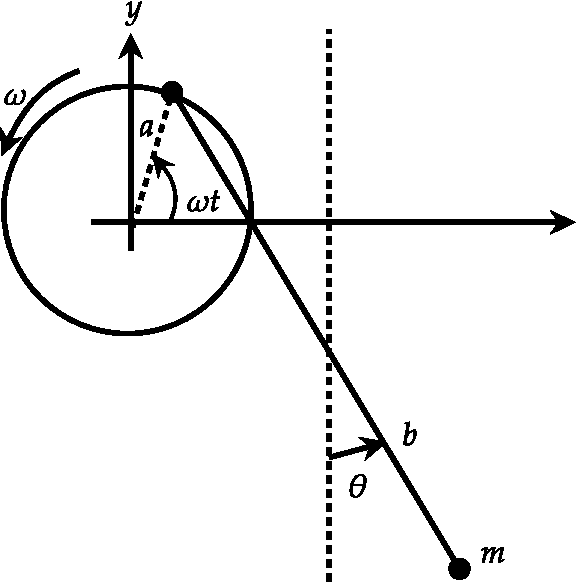
\includegraphics[height=5.5cm,width=5.5cm]{Assignment-HE-05}
	\end{figure}
	\begin{answer}
		\begin{align*}
		\intertext{(a) We choose the origin of our coordinate system to be at the center of the rotating rim. The Cartesian components of mass $m$ become}
		&\left.\begin{array}{l}x=a \cos \omega t+b \sin \theta \\ y=b \cos \theta-a \sin \omega t\end{array}\right\}
		\intertext{The velocities are}
		&\left.\begin{array}{l}\dot{x}=-a w \sin \omega t+b \dot{\theta} \cos \theta \\ \dot{y}=-a \omega \cos \omega t-b \dot{\theta} \sin \theta\end{array}\right\}
		\intertext{Taking the time derivative once again gives the acceleration:}
		\ddot{x}&=-a \omega^{2} \cos \omega t+b\left(\ddot{\theta} \cos \theta-\dot{\theta}^{2} \sin \theta\right)\\
		\ddot{y}&=+a \omega^{2} \sin \omega t-b\left(\ddot{\theta} \sin \theta+\dot{\theta}^{2} \cos \theta\right)
		\intertext{(b) It should now be clear that the single generalized coordinate is $\theta$. The kinetic and potential energies are}
	T &=\frac{1}{2} m\left(\dot{x}^{2}+\dot{y}^{2}\right) \\
	 U &=-m g y \\
	 \text{where }U&=0\text{ at }y=0.
	 \intertext{The Lagrangian of a system is given by}
	 L&=T-U=\frac{m}{2}\left[a^{2} \omega^{2}+b^{2} \dot{\theta}^{2}+2 b \dot{\theta} a \omega \sin (\theta-\omega t)\right]+m g(b \cos \theta-a \sin \omega t)
	 \intertext{(c) The derivatives for the Lagrange equation of motion for $\theta$ are}
	 \frac{d}{d t} \frac{\partial L}{\partial \dot{\theta}}&=m b^{2} \ddot{\theta}+m b a \omega(\dot{\theta}-\omega) \cos (\theta-\omega t)\\
	 \frac{\partial L}{\partial \theta}&=m b \dot{\theta} a \omega \cos (\theta-\omega t)-m g b \sin \theta
	 \intertext{which results in the equation of motion (after solving for $\ddot{\theta}$ )}
	 \ddot{\theta}&=\frac{\omega^{2} a}{b} \cos (\theta-\omega t)-\frac{g}{b} \sin \theta
		\end{align*}
	\end{answer}
	\item $\left. \right. $
	  \begin{figure}[H]
		\centering
		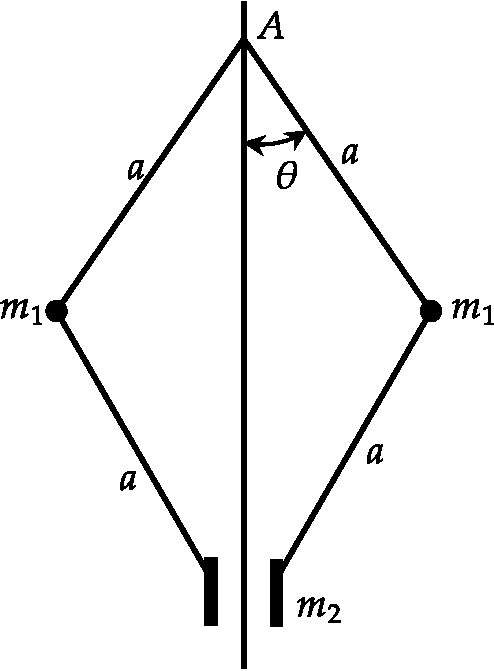
\includegraphics[height=6cm,width=3.6cm]{Assignment-HE-06}
	\end{figure}
	\begin{answer}
		\begin{align*}
		\text{(a) }&r_{1}=a, r_{2}=a, \theta_{1}=\theta_{2}=\theta, \quad \phi_{3}=0, \quad \theta_{3}=0, \quad r_{3}=2 a \cos \theta, \quad \phi_{1}=\phi_{2}+c\\
		&\text{Degree of freedom }=3 \times 3-7=2\\
	\text{	(b) }&L=m_{1} a^{2}\left(\dot{\theta}^{2}+\omega^{2} \sin ^{2} \theta\right)+2 m_{2} a^{2} \dot{\theta}^{2} \sin ^{2} \theta+2\left(m_{1}+m_{2}\right) g a \cos \theta\\
		\text{(c) }&\frac{d}{d t}\left(\frac{\partial L}{\partial \dot{\theta}}\right)-\frac{\partial L}{\partial \theta}=0\\
		&\frac{d}{d t}\left(2 m_{1} a^{2} \dot{\theta}+4 m_{2} a^{2} \dot{\theta} \sin ^{2} \theta\right)-m_{1} a^{2} \omega^{2} 2 \sin \theta \cos \theta-2 m_{2} a^{2} \dot{\theta}^{2} 2 \sin \theta \cos \theta+2\left(m_{1}+m_{2}\right) g a \sin \theta=0\\
		&\Rightarrow\left(2 m_{1} a^{2}+4 m_{2} a^{2} \sin ^{2} \theta\right) \ddot{\theta}+2 m_{2} a^{2} \sin 2 \theta \dot{\theta}^{2}-m_{1} a^{2} \omega^{2} \sin 2 \theta+2\left(m_{1}+m_{2}\right) g a \sin \theta=0\\
	\text{	(d) }&H=\sum \dot{\theta} p_{\theta}-L\\
	&\frac{\partial L}{\partial \dot{\theta}}=p_{\theta}=2 m_{1} a^{2} \dot{\theta}+4 m_{2} a^{2} \dot{\theta} \sin ^{2} \theta \Rightarrow \dot{\theta}=\frac{p_{\theta}}{2 m_{1} a^{2}+4 m_{2} a^{2} \sin ^{2} \theta}\\
	H&=\frac{p_{\theta}^{2}}{4 m a^{2}+\theta m_{2} a^{2} \sin ^{2} \theta}-m_{1} a^{2} \omega^{2} \sin ^{2} \theta-2\left(m_{1}+m_{2}\right) g a \cos \theta
		\end{align*}
	\end{answer}
	\item $\left. \right. $
	 \begin{figure}[H]
		\centering
		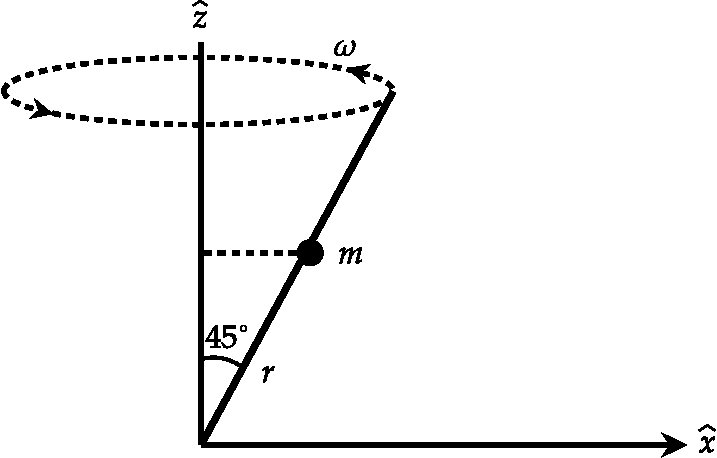
\includegraphics[height=4.5cm,width=6.5cm]{Assignment-HE-07}
	\end{figure}
	\begin{answer}
		\begin{align*}
		L&=\frac{1}{2} m\left(\dot{r}^{2}+r^{2} \dot{\theta}^{2}+r^{2} \sin ^{2} \theta \dot{\phi}^{2}\right)-m g r \cos \theta\\
		\text{equation of constrain is }\theta&=\frac{\pi}{4}\text{ and it is given }\dot{\phi}=\omega\\
		L&=\frac{1}{2} m\left(\dot{r}^{2}+\frac{1}{2} r^{2} \omega^{2}\right)-\frac{1}{\sqrt{2}} m g r\\
	\text{	the momentum conjugate to $r$ is }p_{r}&=\frac{\partial L}{\partial \dot{r}} \quad \Rightarrow p_{r}=m \dot{r}
		\end{align*}
	\end{answer}
		\item $\left. \right. $
		  \begin{figure}[H]
			\centering
			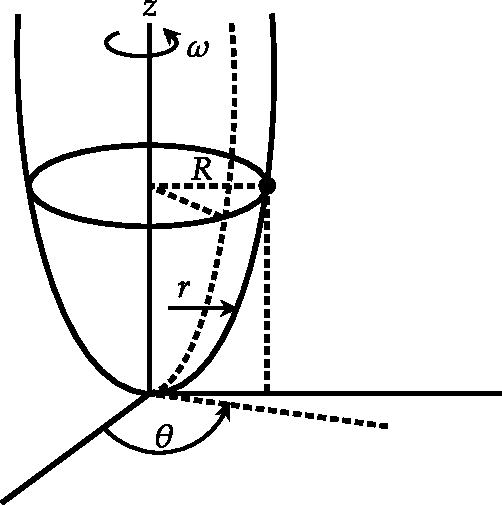
\includegraphics[height=6cm,width=5.2cm]{Assignment-HE-08}
		\end{figure}
	\begin{answer}
		\begin{align}
		\intertext{Because the problem has cylindrical symmetry, we choose $r, \theta$ and $z$ as the generalized coordinates. The kinetic energy of the bead is}
		T&=\frac{m}{2}\left[\dot{r}^{2}+\dot{z}^{2}+(r \dot{\theta})^{2}\right]\notag\\
	\text{	If we choose }U=0\text{ at }z&=0\text{, the potential energy term is}\notag\\
	U&=m g z\notag
	\intertext{But $r, z$ and $\theta$ are not independent. The equation of constraint for the parabola is}
	z&=c r^{2} \Rightarrow \dot{z}=2 c \dot{r} r\notag
	\intertext{We also have an explicit time dependence of the angular rotation}\notag
	\theta&=\omega t \Rightarrow \dot{\theta}=\omega\notag
	\intertext{We can now construct the Lagrangian as being dependent only on $r$, because there is no direct $\theta$ dependence.}
	L&=T-U=\frac{m}{2}\left(\dot{r}^{2}+4 c^{2} r^{2} \dot{r}^{2}+r^{2} \omega^{2}\right)-m g c r^{2}\notag
	\intertext{The problem stated that the bead moved in a circle of radius $R$. The reader might be tempted at this point to let $r=R=$ constant and $\dot{r}=0$. It would be a mistake to do this now in the Lagrangian. First, we should find the equation of motion for the variable $r$ and then let $r=R$ as a condition of the particular motion. This determines the particular value of $c$ needed for $r=R$.}\notag
	\frac{\partial L}{\partial \dot{r}}&=\frac{m}{2}\left(2 \dot{r}+8 c^{2} r^{2} \dot{r}\right), \frac{d}{d t} \frac{\partial L}{\partial \dot{r}}=\frac{m}{2}\left(2 \ddot{r}+16 c^{2} r \dot{r}^{2}+8 c^{2} r^{2} \ddot{r}\right)\notag\\
	\frac{\partial L}{\partial \dot{r}}&=m\left(4 c^{2} r \dot{r}^{2}+r \omega^{2}-2 g c r\right)\notag
	\intertext{Lagrange's equation of motion becomes}\notag\\
	\ddot{r}\left(1+4 c^{2} r^{2}\right)&+\dot{r}^{2}\left(4 c^{2} r\right)+r\left(2 g c-\omega^{2}\right)=0\label{HE-01}
	\intertext{which is a complicated result. If, however, the bead rotates with $r=R=$ constant, then $\dot{r}=\ddot{r}=0$ and equation (\ref{HE-01}) becomes}
	R\left(2 g c-\omega^{2}\right)&=0 \Rightarrow \omega=\sqrt{2 g c}\notag
		\end{align}
	\end{answer}
\end{enumerate}
\begin{abox}
	Assignment solution-2
\end{abox}
\begin{enumerate}
	\item 
	
	
	
	
\end{enumerate}